\section{Μοντέλα CNN}
\label{sec:cnn_impl}

Όπως αναφέραμε \autoref{sec:dnn_sw} το βασικό εργαλείο λογισμικού που
χρησιμοποιήσαμε για την ανάπτυξη των μοντέλων CNN είναι το \emph{Keras}.

Η βιβλιοθήκη Keras προσφέρει τις υλοποιήσεις όλων των επιπέδων που
απαιτούνται για για την ανάπτυξη ενός CNN
\footnote{Πλήρες περιγραφή της λίστας των διαθέσιμων επιπέδων: \href{https://keras.io/layers/core/}{https://keras.io/layers/core/}}.
Πιο συγκεκριμένα, τα επίπεδα που χρησιμοποιήθηκαν, καθώς και οι βασικές
παράμετροι τους περιγράφονται πιο κάτω:
\begin{itemize}
  \item{\textbf{InputLayer}: Επίπεδο Εισόδου του νευρωνικού δικτύου}
    \begin{itemize}
      \item{Διαστάσεις του όγκου εισόδου (tensor shape)}
    \end{itemize}
  \item{Convolution2D: Επίπεδο Συνέλιξης}
    \begin{itemize}
      \item{Μορφολογία της εισόδου}
      \item{Αριθμός των φίλτρων συνέλιξης}
      \item{Διαστάσεις των φίλτρων συνέλιξης}
      \item{Συνάρτηση ενεργοποίησης}
    \end{itemize}
  \item{MaxPooing2D: Επίπεδο Υποδειγματοληψίας}
    \begin{itemize}
      \item{Διαστάσεις πλαισίου}
      \item{Βήμα μετατόπισης}
    \end{itemize}
  \item{ZeroPadding2D: Προσθέτει πλαίσιο με μηδενικά στον όγκο εισόδου}
    \begin{itemize}
      \item{Διαστάσεις του πλαισίου}
    \end{itemize}
  \item{Activation: Επίπεδο ενεργοποίησης. Εφαρμόζει συνάρτηση ενεργοποίησης στον
    όγκο εξόδου του προηγούμενου επιπέδου}
  \item{Dropout: Επίπεδο πρόληψης υπέρ-προσαρμογής \cite{lecun2015deep}}
  \item{Dense: Πλήρες συνδεδεμένο επίπεδο}
    \begin{itemize}
      \item{Διαστάσεις του όγκου εισόδου (Προαιρετικό)}
      \item{Διαστάσεις του όγκου εξόδου}
      \item{Συνάρτηση ενεργοποίησης}
    \end{itemize}
  \item{Flatten: Μετασχηματίζει τον όγκου εισόδου σε επίπεδη αναπαράσταση
    (π.χ. για όγκο εισόδου $64 \times 32 \times 32$ η έξοδος θα είναι επίπεδη με $65536$ νευρώνες}
  \item{BatchNormalization: Εφαρμόζει μετασχηματισμό για να κρατήσει την μέση τιμή
      και την τυπική απόκλιση των ενεργοποιήσεων του προηγούμενου επιπέδου στις τιμές 0 και 1 αντίστοιχα}
\end{itemize}

Σημαντική παρατήρηση είναι το γεγονός ότι η επιστήμη της βαθιάς μηχανικής μάθησης
βρίσκεται σε πρώιμο στάδιο, με αποτέλεσμα να μην υπάρχουν συγκεντρωμένες
οι υλοποιήσεις των διαφόρων επιπέδων και γενικότερα των μοντέλων σύγχρονων ΑNN.

Περαιτέρω, η επιλογή των μοντέλων CNN για ανάπτυξη στηρίχθηκε στην ύπαρξη και
προ-εκπαιδευμένων βαρών για τα αντίστοιχα CNN στο διαδίκτυο για 2 λόγους:
\begin{itemize}
  \item{Η διαδικασία εκπαίδευσης είναι χρονοβόρα διαδικασία και προϋποθέτει
    τη χρησιμοποίηση μίας ή περισσοτέρων ισχυρών μονάδων GPU (NVIDIA Titam X GPU)}
  \item{Η εκπαίδευση νευρωνικών δικτύων ξεφεύγει από τα πλαίσια της παρούσας
    διπλωματικής εργασίας}
\end{itemize}


\subsection{AlexNet}

Το δίκτυο AlexNet ήταν η αρχή της εισαγωγής της βαθιάς
μηχανικής μάθησης στην επιστήμη της μηχανικής όρασης. Χρησιμοποιήθηκε
στον διαγωνισμό ImageNet ILSVRC challenge, το 2012, κερδίζοντας με διαφορά
10,9\%, στο σφάλμα αναγνώρισης αντικειμένων σε σύνολο 1000 κλάσεων.

\begin{figure}[!ht]
  \centering
  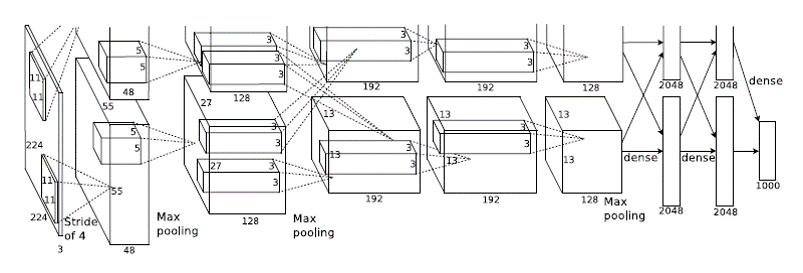
\includegraphics[width=1\textwidth]{./images/chapter5/alexnet_from_paper.png}
  \caption[Κλάδοι και εφαρμογές της επιστήμης της Τεχνητής Νοημοσύνης]{Κλάδοι και εφαρμογές της επιστήμης της Τεχνητής Νοημοσύνης}
  \label{fig:ai_1}
\end{figure}

Το συγκεκριμένο νευρωνικό δίκτυο συνέλιξης αποτελείται από σύνολο οκτώ επίπεδα;
πέντε επίπεδα συνέλιξης και 3 πλήρως συνδεδεμένα. \\

\begin{tabular}{ | l | l | l | l | }
  \hline
  \rowcolor{Gray}
  Επίπεδο  & Τύπος & Αριθμός καναλιών & Διαστάσεις φίλτρων \\
  \hline
  1 & Conv+Max+Norm & 96 & $11 \times 11$ \\
  2 & Conv+Max+Norm & 256 & $5 \times 5$ \\
  3 & Conv & 384 & $3 \times 3$ \\
  4 & Conv & 384 & $3 \times 3$ \\
  5 & Conv+Max & 256 & $3 \times 3$ \\
  6 & Full & 4096 & Ν/A \\
  7 & Full & 4096 & N/A \\
  8 & Full & 1000 & N/A \\
  \hline
\end{tabular}
\\

Σε όλα τα επίπεδα εκτός του τελευταίου χρησιμοποιήθηκε η συνάρτηση ενεργοποίησης
ReLU. Το τελευταίο επίπεδο παίζει τον ρόλο του ταξινομητή και συγκεκριμένα
είναι ένας ταξινομητής Softmax.
Επίσης χρησιμοποιεί και πολλά επίπεδα ZeroPadding με πλαίσιο
διαστάσεων $1 \times 1$. Ο αντίστοιχος γράφος της υλοποίησης του μοντέλου
φαίνεται φαίνεται στο \autoref{fig:alexnet_2}.

\begin{figure}[!ht]
  \centering
  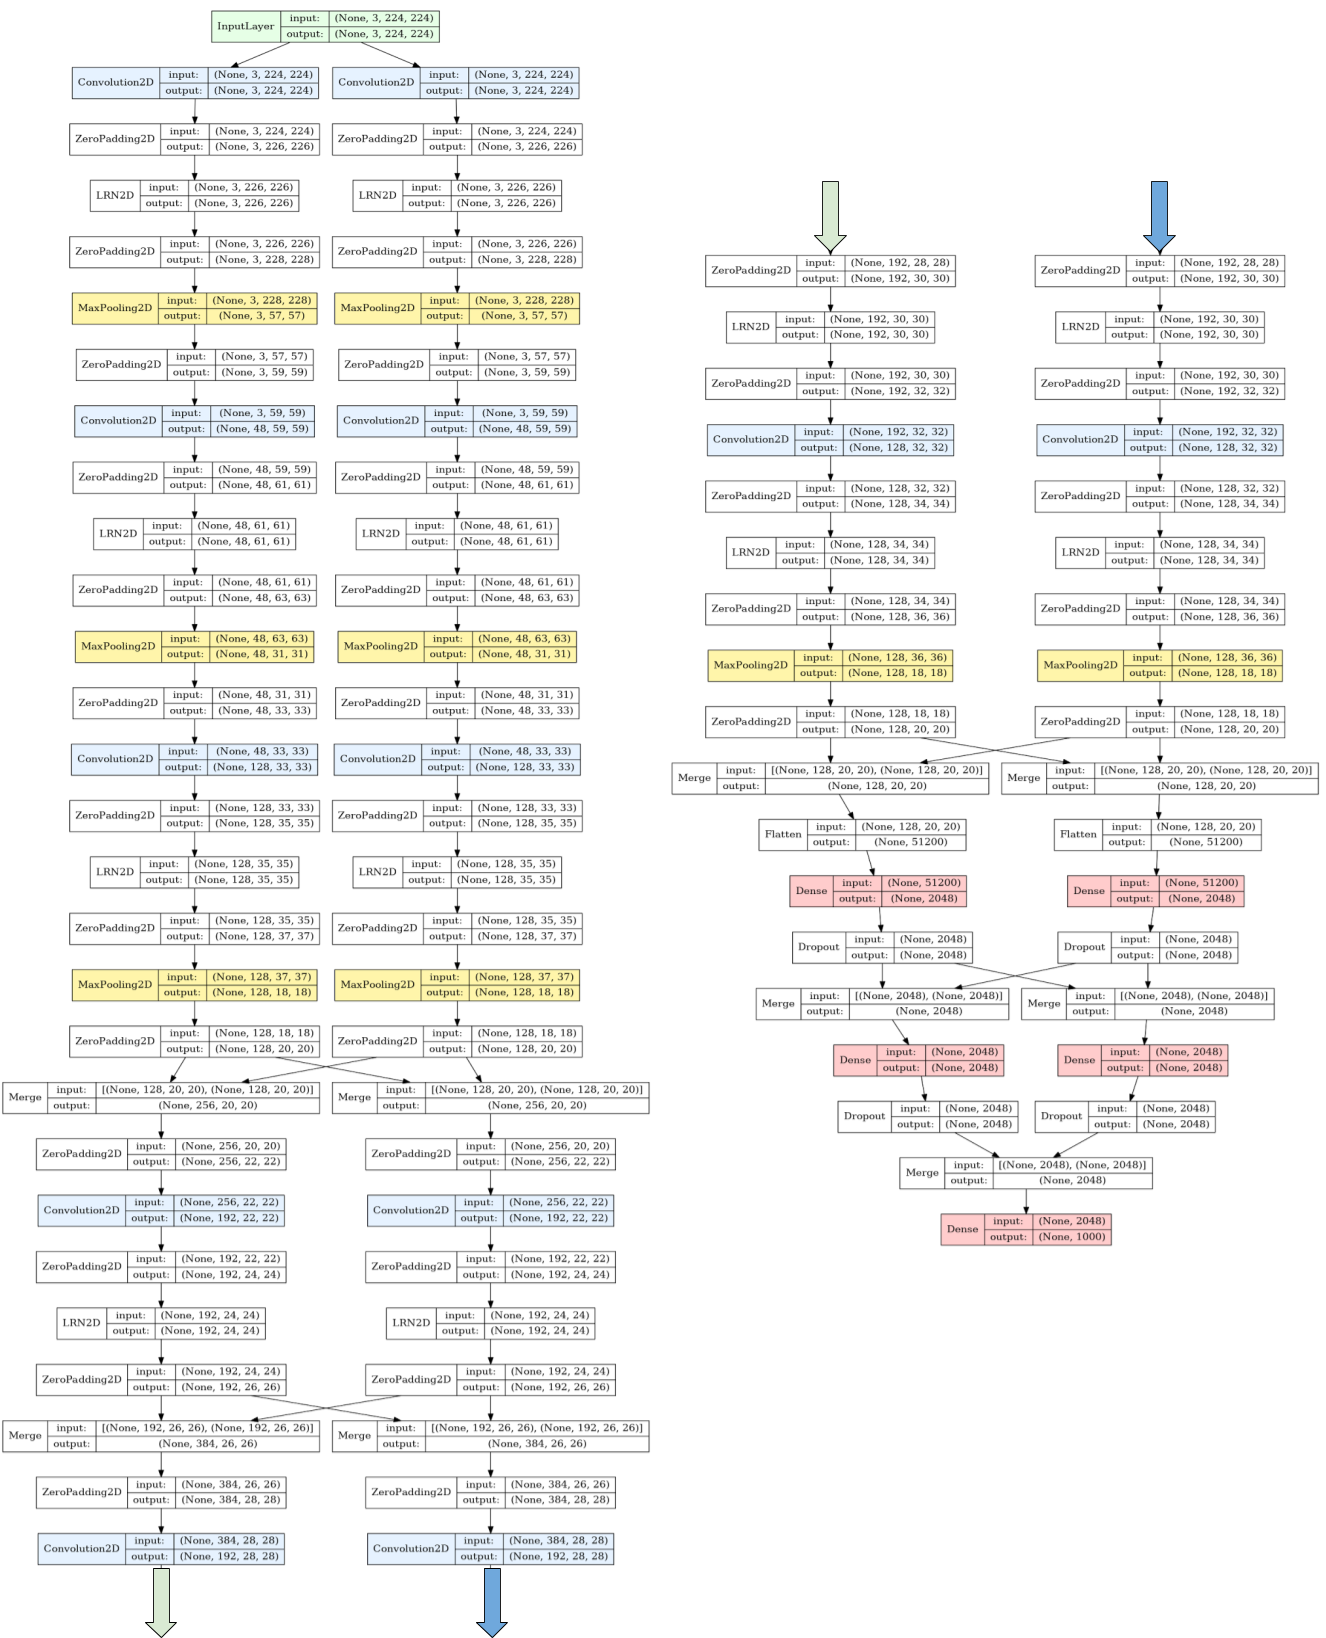
\includegraphics[width=0.8\textwidth]{./images/chapter5/alexnet_3.png}
  \caption[Κλάδοι και εφαρμογές της επιστήμης της Τεχνητής Νοημοσύνης]{Κλάδοι και εφαρμογές της επιστήμης της Τεχνητής Νοημοσύνης}
  \label{fig:alexnet_2}
\end{figure}

Το AlexNet είναι ένα μοντέλο μόνο για αναγνώριση και όχι για εντοπισμό
των αντικειμένων, δηλαδή η μόνη πληροφορία που μας δίνει είναι η κλάση των
αντικειμένων.

\subsection{VGG16}

\begin{tabular}{ | l | l | l | l | }
  \hline
  \rowcolor{Gray}
  Επίπεδο  & Τύπος & Αριθμός καναλιών & Διαστάσεις φίλτρων \\
  \hline
  1 & conv+max+norm & 96 & $11 \times 11$ \\
  2 & conv+max+norm & 256 & $5 \times 5$ \\
  3 & conv+max+norm & 384 & $3 \times 3$ \\
  4 & conv+max+norm & 384 & $3 \times 3$ \\
  5 & conv+max+norm & 256 & $3 \times 3$ \\
  6 & conv+max+norm & 4096 & Ν/A \\
  7 & conv+max+norm & 4096 & N/A \\
  8 & conv+max+norm & 1000 & N/A \\
  \hline
\end{tabular}

\begin{figure}[!ht]
  \centering
  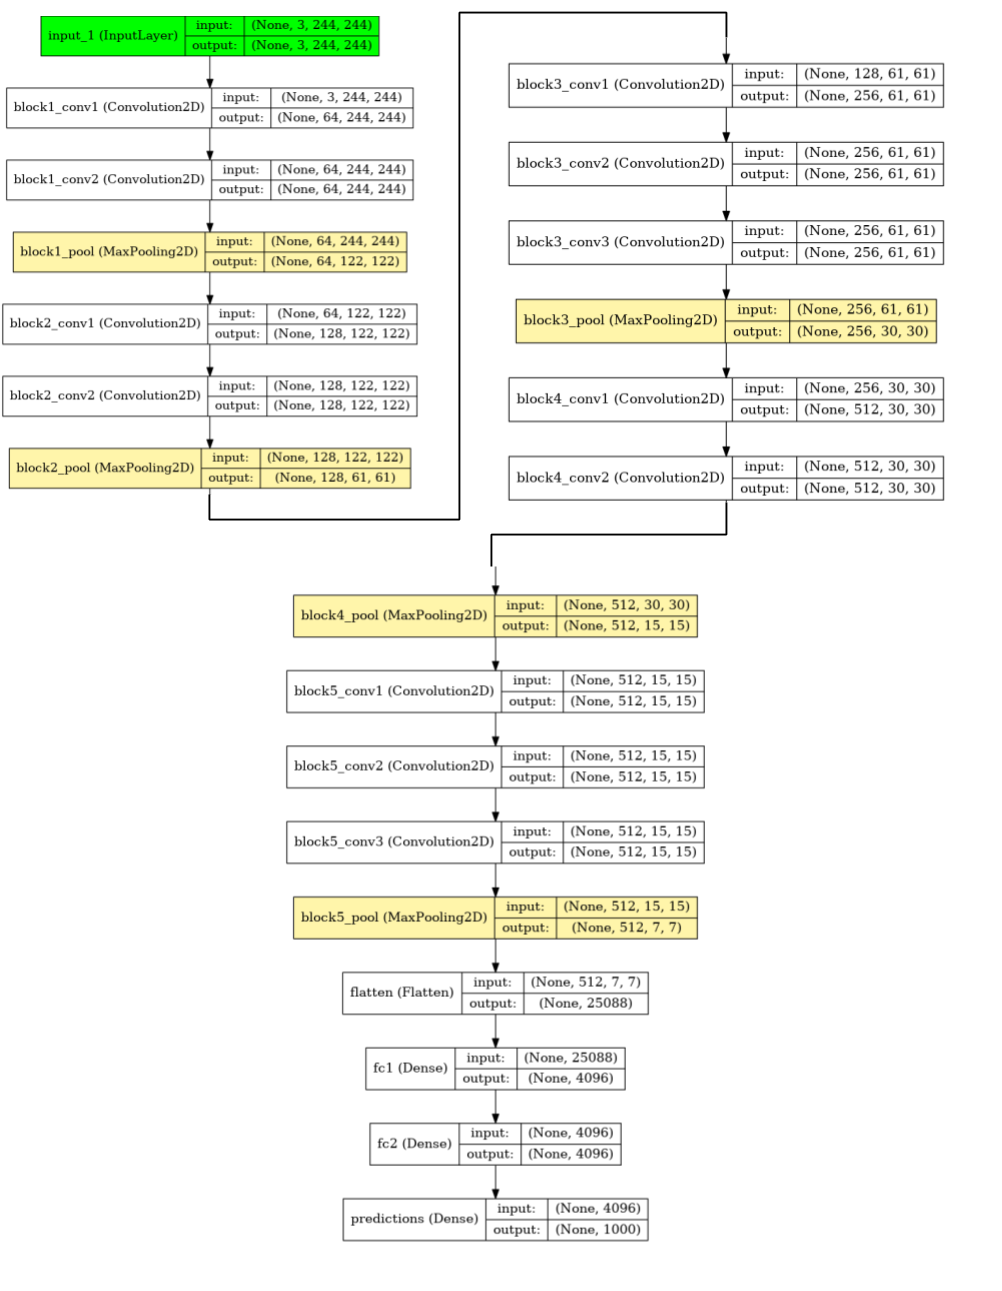
\includegraphics[width=1\textwidth]{./images/chapter5/vgg16.png}
  \caption[Κλάδοι και εφαρμογές της επιστήμης της Τεχνητής Νοημοσύνης]{Κλάδοι και εφαρμογές της επιστήμης της Τεχνητής Νοημοσύνης}
  \label{fig:vgg16}
\end{figure}

\subsection{VGG19}

\subsection{GoogleNet aka Inception-V1}
